\documentclass[11pt,fleqn]{article}
\usepackage[margin=1in]{geometry}
\usepackage{tikz}
\usepackage{mathtools}
\usepackage{longtable}
\usepackage{enumitem}
\usepackage[colorlinks = true,
		linkcolor=black,
		citecolor=black,
	        urlcolor  = black]{hyperref}
%\usepackage[dvips]{graphics}
%\usepackage[table]{xcolor}
%\usepackage{amssymb}
\usepackage{float}
%\usepackage{subfig}
\usepackage{booktabs}
\usepackage{subcaption}
\usepackage{booktabs}

\usepackage[normalem]{ulem}

\usepackage{multicol}
\usepackage{txfonts}
\usepackage{amsfonts}
\usepackage{natbib}

\usepackage{multirow}

\usepackage{gb4e}
\usepackage[all]{xy}
\usepackage{rotating}
\usepackage{tipa}
\usepackage{multirow}
\usepackage{authblk}
\usepackage{url}
\usepackage{pdflscape}
\usepackage{rotating}
\usepackage{adjustbox}
\usepackage{array}

\usepackage{dcolumn} % for printing model output tables directly from R

\usepackage{graphics}
\graphicspath{{../../results/MegaVeridicality/graphs/}}

%\usepackage{color}
%\DeclareOuterCiteDelims{cite}{\textcolor{green}{\bibopenbracket}}{\textcolor{red}{\bibclosebracket}}

\definecolor{Pink}{RGB}{255,50,170}
\newcommand{\jd}[1]{\textcolor{Pink}{[jd: #1]}}  

\newcommand{\jt}[1]{\textbf{\color{purple}JT: #1}}

\newcommand{\tableref}[1]{Tab.~\ref{#1}}
\newcommand{\figref}[1]{Fig.~\ref{#1}}

\def\bad{{\leavevmode\llap{*}}}
\def\marginal{{\leavevmode\llap{?}}}
\def\verymarginal{{\leavevmode\llap{??}}}
\def\swmarginal{{\leavevmode\llap{4}}}
\def\infelic{{\leavevmode\llap{\#}}}

\definecolor{airforceblue}{rgb}{0.36, 0.54, 0.66}
%\definecolor{gray}{rgb}{0.36, 0.54, 0.66}

\newcommand{\dashrule}[1][black]{%
  \color{#1}\rule[\dimexpr.5ex-.2pt]{4pt}{.4pt}\xleaders\hbox{\rule{4pt}{0pt}\rule[\dimexpr.5ex-.2pt]{4pt}{.4pt}}\hfill\kern0pt%
}

\setlength{\parindent}{.3in}
\setlength{\parskip}{0ex}

\newcommand{\yi}{\'{\symbol{16}}}
\newcommand{\nasi}{\~{\symbol{16}}}
\newcommand{\hina}{h\nasi na}
\newcommand{\ina}{\nasi na}

\newcommand{\foc}{$_{\mbox{\small F}}$}

\hyphenation{par-ti-ci-pa-tion}

%\setlength{\bibhang}{0.5in}
%\setlength{\bibsep}{0mm}
%\bibpunct[:]{(}{)}{,}{a}{}{,}

\newcommand{\6}{\mbox{$[\hspace*{-.6mm}[$}} 
\newcommand{\9}{\mbox{$]\hspace*{-.6mm}]$}}
\newcommand{\sem}[2]{\6#1\9$^{#2}$}
\renewcommand{\ni}{\~{\i}}

\newcommand{\citepos}[1]{\citeauthor{#1}'s (\citeyear{#1})}
\newcommand{\citeposs}[1]{\citeauthor{#1}'s}
\newcommand{\citetpos}[1]{\citeauthor{#1}'s \citeyear{#1}}

\newcolumntype{R}[2]{%
    >{\adjustbox{angle=#1,lap=\width-(#2)}\bgroup}%
    l%
    <{\egroup}%
}
\newcommand*\rot{\multicolumn{1}{R{90}{0em}}}% no optional argument here, please!

\title{How do the entailments of a \emph{that}-clause-embedding predicate modulate the projection of its CC?}

\author{YK}

\begin{document}

\maketitle

\section{The gist}
\begin{itemize}
\item Traditionally, projection of the CC of a \emph{that}-clause-embedding predicates is explained in terms of factivity: if a predicate is factive, its CC is presupposed and therefore projects; if it non-factive, the CC does not project (\citealt{kiparsky-kiparsky70}). 
\item However, the categorical factive/non-factive distinction does not predict the projection ratings obtained in experiments, which show high levels of variability (\citealt{degen-tonhauser-language}). 
\item The predicate type (cognitive, communicative, emotive, evidential) is another category that predicts projection ratings to some extent. However, within each type we again observe high variability, including within those predicate types thought to reflect the factive/non-factive distinction, i.e., the emotives, considered mostly factive, and the communicatives, considered generally non-factive (\citealt{anand-hacquard2014}).
\item A good starting point for trying to find an explanation for the observed variability are the communicatives, precisely because their CC is not predicted to project and yet often does, with some of these predicates receiving even higher projection ratings than the factive fan favourite \emph{know} (\citealt{white-rawlins-nels2018}). 
\item As White and Rawlins’s (2018) participants provided their ratings based on “low-content items” without any context, it is reasonable to assume that the differences in projection ratings in the MegaVeridicality dataset are the result of differences in the lexical meaning of these communicative predicates. 
\item Since the meaning of a clause embedding predicate can be defined as the set of its entailments, in order to better understand if and how the meaning of these predicates modulates projection, a closer examination of their entailments is required.
To this end, I am going to collect ratings on the entailments of communicative predicates and the projection of their CC.
\end{itemize}

\section{Predicates}
\subsection{The MegaVeridicality dataset}
The starting point for this investigation is \citepos{white-rawlins-nels2018} MegaVeridicality (MV) dataset, which contains veridicality judgements for 517 predicates, 348 of which occur in an``active frame" and 142 in a ``passive frame", containing either passivised verbal predicates, like be advised or adjectival predicates, such as be delighted. The 27 predicates that occur in both frames are considered separately for each of them, resulting in a total number of 544 predicates. 
\begin{itemize}
	\item Stimuli: \citepos{white-rawlins-nels2018} participants saw either utterances as in (1) below, which were followed by the question “Did that thing happen?”, or as in (2), in which the question was already included.
	\begin{exe}		
		\ex 
		\begin{xlist}
			\ex Someone \{thought, didn’t think\} that a particular thing happened.
			\ex Someone \{was, wasn’t\} told that a particular thing happened. \hfill(\citealt{white-rawlins-nels2018})
		\end{xlist}
	\end{exe}

	\begin{exe}		
		\ex 
		\begin{xlist}
			\ex If someone \{did, didn’t\} know that a particular thing happened, did that thing happen?
			\ex If someone \{was, wasn’t\} told that a particular thing happened, did that thing happen? \\ \null\hfill(\citealt{white-rawlins-nels2018}, slightly modified)
		\end{xlist}
	\end{exe}
	\item Projection ratings in the MV dataset are therefore based on three different environments, with the predicates embedded under different (combinations of) entailment-cancelling operators: negation, the antecedent of a conditional and a polar question, or a combination of all three operators. 
	\item \cite{white-rawlins-nels2018} asked their participants to answer ``yes", ``maybe or maybe not" or ``no". These responses were recoded as 1, 0 and -1, respectively.
	\item The MV dataset furthermore includes acceptability ratings given by participants on a 7-point Likert scale for each utterance they evaluated.
\end{itemize}

\subsection{Classification of predicates}
\begin{itemize}
	\item Because many of the predicates in the MV dataset can take on different meanings depending on how they are used, my classifications of these predicates are strictly based on their meaning in the stimuli used by \cite{white-rawlins-nels2018}. 
	\begin{itemize}
		\item The predicates in the MV dataset only occur in the past tense, therefore all classifications regarding their lexical meaning are based solely on their use in the past tense. 
		\item The meaning of the predicates was only considered in the context of the specific “low lexical content” complement clause used by \cite{white-rawlins-nels2018}.	
	\end{itemize}
	\item The main distinction made for this investigation is that between communicative and private predicates.
	\begin{itemize}
		\item A predicate \emph{P} is communicative if and only if ``\emph{X} \emph{P}ed that \emph{m}" requires \emph{X} to have externalised \emph{m}. This externalisation may be have been verbal or nonverbal. 
		\item A predicate \emph{P} is private if and only if ``\emph{X} \emph{P}ed that \emph{m}" conveys that \emph{m} stands in some relation to \emph{X}'s mental representation of the world. \emph{X} does not have to believe that \emph{m} is true.
	\end{itemize}
	\item Amongst the private predicates I distinguish between three subtypes: cognitives, emotives and evidentials. 
	\begin{itemize}
		\item A predicate \emph{P} is cognitive if and only if ``\emph{X} \emph{P}ed that \emph{m}" conveys something about \emph{X}'s relation to \emph{m}.
		\item A predicate \emph{P} is emotive if and only if ``\emph{X} \emph{P}ed that \emph{m}" conveys that \emph{X} has a feeling or emotion towards \emph{m}. 
		\item A predicate \emph{P} is evidential if and only if ``\emph{X} \emph{P}ed that \emph{m}" conveys the source of information by which \emph{X} received the information about \emph{m}.
	\end{itemize}
	\item 12 predicates that can be used both as communicative and private predicates were excluded from analysis, as well as the 29 predicates that could not be assigned to any of the predicate types, leaving 503 predicates, including 217 communicatives.
	\item Because of a strong positive correlation between acceptability ratings and projection ratings, only the 474 predicates with a mean acceptability rating of greater than 4 (midpoint of the scale) are included in my analysis, 201 of which are communicatives.
\end{itemize}

\section{Entailments of communicatives}
\subsection{Emotion entailment}
\subsubsection{Classification}
\figref{projpredtype} shows that the mean projection rating of the emotives in the MV dataset is much higher than that of the other predicate types defined above.

\begin{figure}[H]
	\centering
	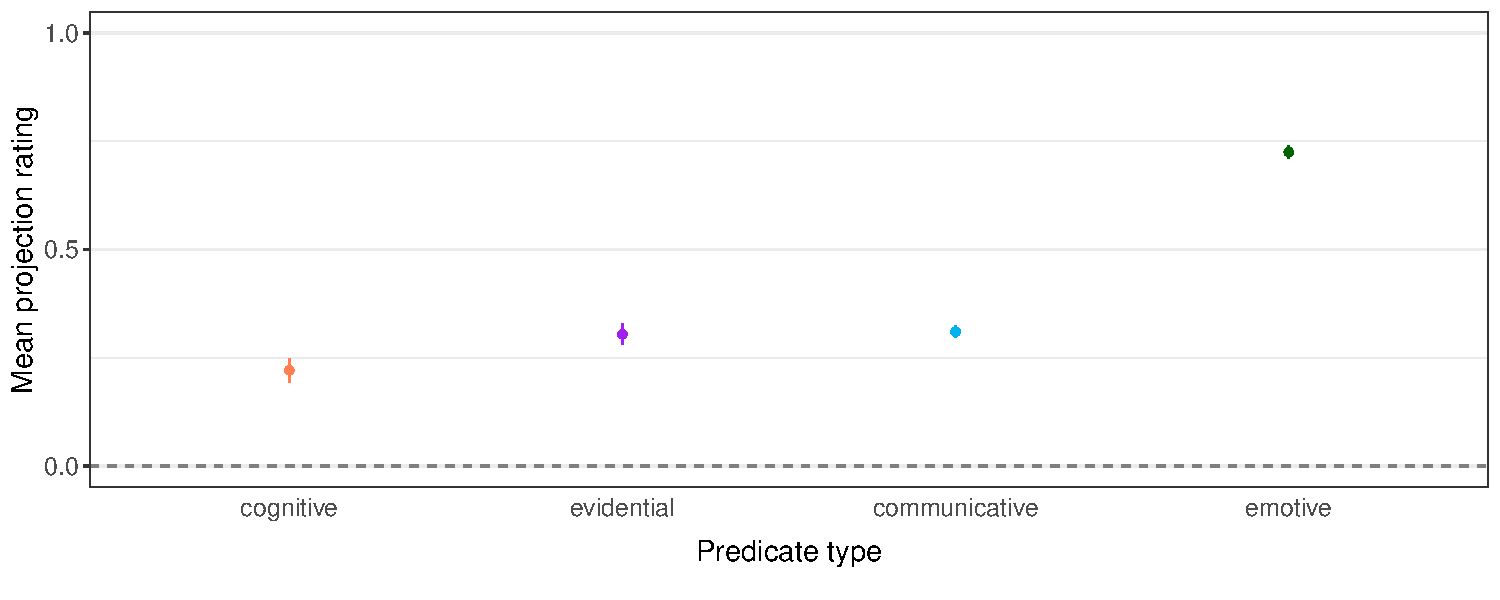
\includegraphics[width=1\textwidth]{projection-by-predicateType}
	\caption{Mean projection rating by predicate type.}
	\label{projpredtype}
\end{figure}

Because the emotives were found to be more projective overall than predicates of the other types, the communicative predicates were subcategorised depending on whether they have an ‘emotion entailment’ or not. Communicatives with an `emotion entailment' entail that the subject has an emotion / a feeling about the CC. That this is in fact an entailment can be confirmed with the defeasibility and reinforcement diagnostics:

\begin{exe}
	\ex
	\begin{xlist}
		\ex [\#] {John groaned that a particular thing happened, but he had no emotion/feeling about the matter.}
		\ex [\#] {John groaned that a particular thing happened, and he had some emotion/feeling about the matter.}
	\end{xlist}
\end{exe}
As (1a) is contradictory and (1b) sounds redundant, the subject’s having an emotion/feeling is an entailment of the predicate.

\figref{projpredtype2} shows that the mean projection rating of the 27 communicatives with an emotion entailment, although not nearly as high as for the emotives, is significantly higher than that of the cognitives, evidentials and communicatives without an emotion entailment.

\begin{figure}[H]
	\centering
	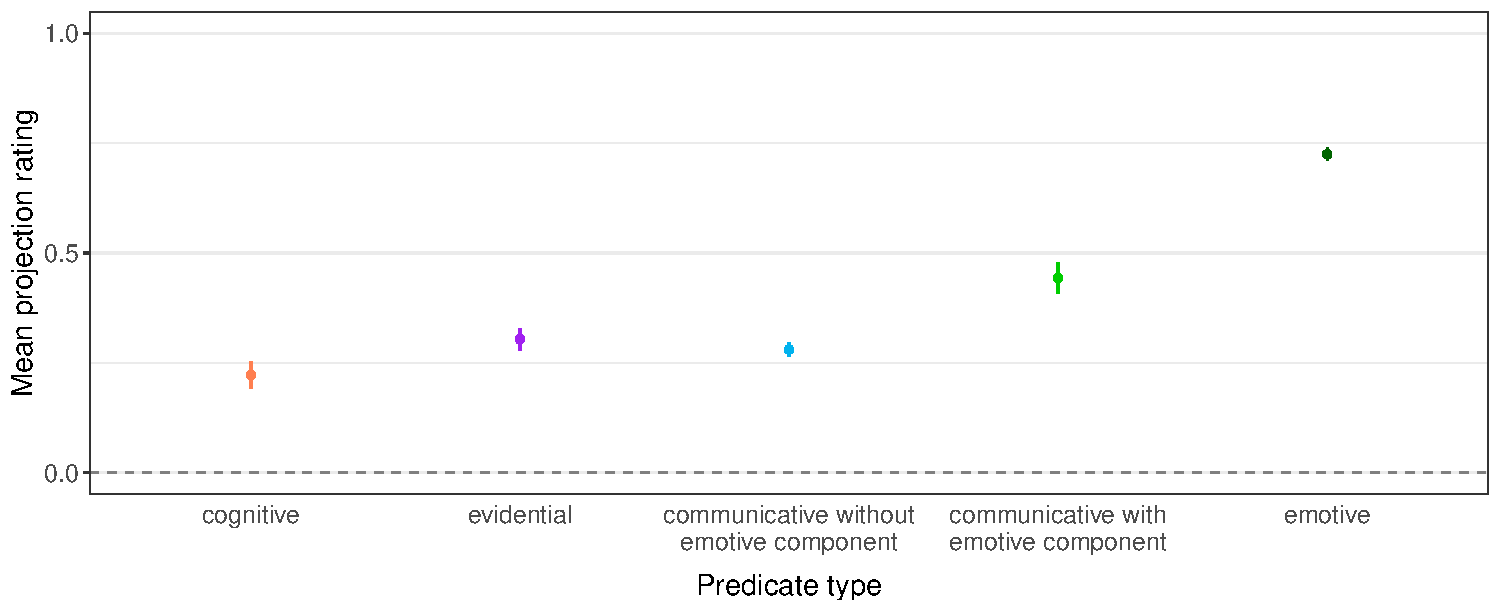
\includegraphics[width=1\textwidth]{projection-by-predicateType2}
	\caption{Mean projection rating by predicate type with distinction between communicatives with and without an emotion entailment.}
	\label{projpredtype2}
\end{figure}

\subsubsection{Measures of emotivity}
That the quality identified by the diagnostics above is indeed emotion and not merely an attitude towards the CC is supported by an investigation of ratings of emotional valence, arousal and dominance (VAD) for the predicates in question, as these are the three measures that are traditionally considered to make up emotions (\citealt{warriner-etal2013}). \citepos{warriner-etal2013} collection of valence, arousal and dominance ratings for 13,915 English lemmas contains ratings for 388 of the predicates in the MV dataset that are part of the present investigation, including 177 communicatives, 25 of which have an emotion entailment.
\begin{itemize}
	\item Original ratings: \citepos{warriner-etal2013} participants provided their ratings on scales of 1 to 9, ranging from 
	\begin{itemize}
		\item Valence: completely unhappy to completely happy.
		\item Arousal: completely calm to completely aroused.
		\item Dominance: Completely controlled to completely in control.
	\end{itemize}
	\item Rescaled ratings: the researchers suggest that on all three scales, a rating of 5 would indicate a neutral state. However, whilst valence and dominance do in fact have a neutral state between the extremes, the neutral state of arousal is not in the middle of the ``calm – aroused" scale, but at its lower end: calmness is the absence of arousal; there is no such thing as ‘negative’ arousal. 
	\item Hence, for this investigation
	\begin{itemize}
		\item Valence and dominance ratings are converted into absolute values of their distance from the neutral state and the direction of this distance is recorded as an additional variable. 
		\item The ratings for all three measures are rescaled to range from 0 to 1. On this new scale, 0 indicates neutrality and 1 indicates the highest level of emotional valence, arousal or dominance.
	\end{itemize}
\end{itemize}
As \figref{VADpredtype} shows, for communicatives with an emotion entailment, valence and arousal ratings are much higher than for those without it. Furthermore, arousal ratings of the communicatives with an emotion entailment are like those of the emotives, i.e., the difference between the mean arousal ratings for these two predicate types is not statistically significant. The similarity of this subgroup of communicatives with the emotives in this respect suggest that they share some of their meaning, specifically the fact that the attitude holder/subject is emotionally affected by the CC.

\begin{figure}[H]
	\centering
	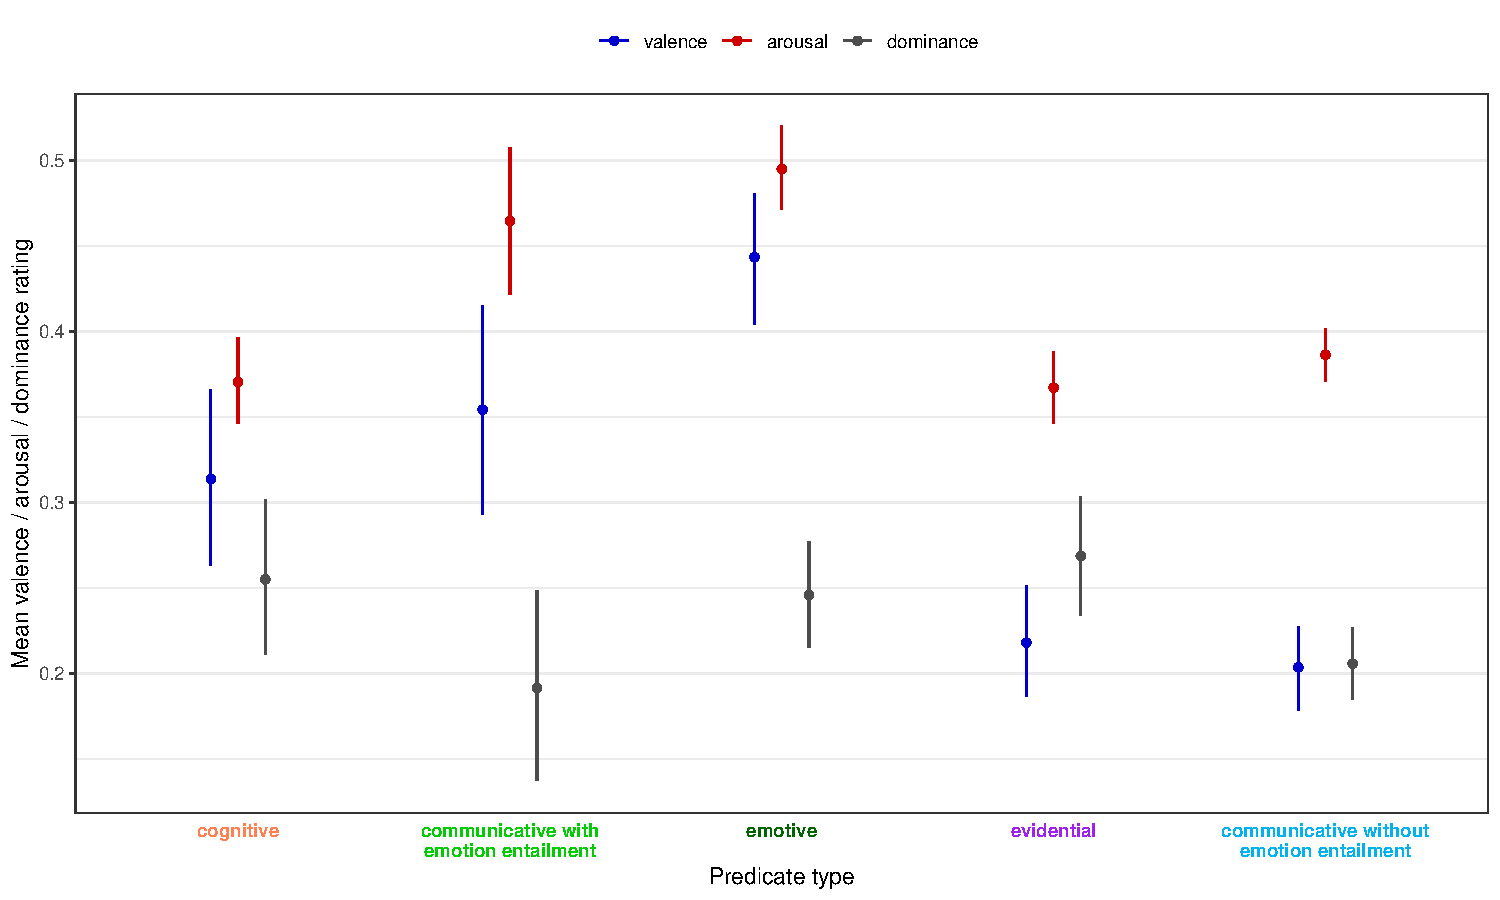
\includegraphics[width=1\textwidth]{valence-arousal-dominance-by-predicateType2-2}
	\caption{Mean valence/arousal/dominance rating by predicate type.}
	\label{VADpredtype}
\end{figure}

Further down the line, when the entailment structures of these predicates are defined and related to their projection ratings, VAD ratings may provide more detailed explanations for the differences in projection ratings between individual predicates within the investigated subgroups in several ways:

Across all predicate types, higher valence and arousal ratings are associated with higher projection ratings, as shown in \figref{projVADdir} below.

\begin{figure}[H]
	\centering
	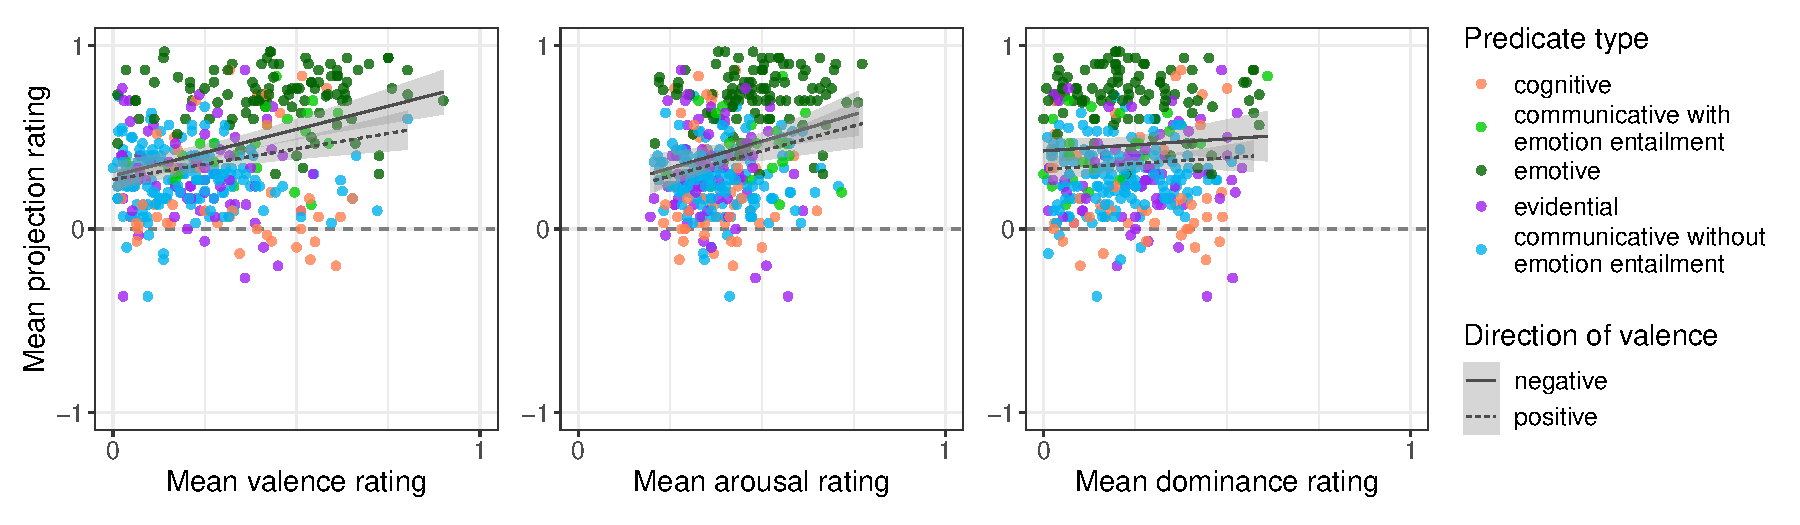
\includegraphics[width=1\textwidth]{projection-by-VAD-with-direction-of-valence}
	\caption{Mean projection rating by mean valence/arousal/dominance rating with separate fitted lines for predicates with negative and positive valence.}
	\label{projVADdir}
\end{figure}

Amongst the communicatives, however, only the correlation of valence and projection ratings is significant. \figref{projvalfac} shows that the positive correlation between valence and projection ratings is only significant for those communicatives with an emotion entailment. 

\begin{figure}[H]
	\centering
	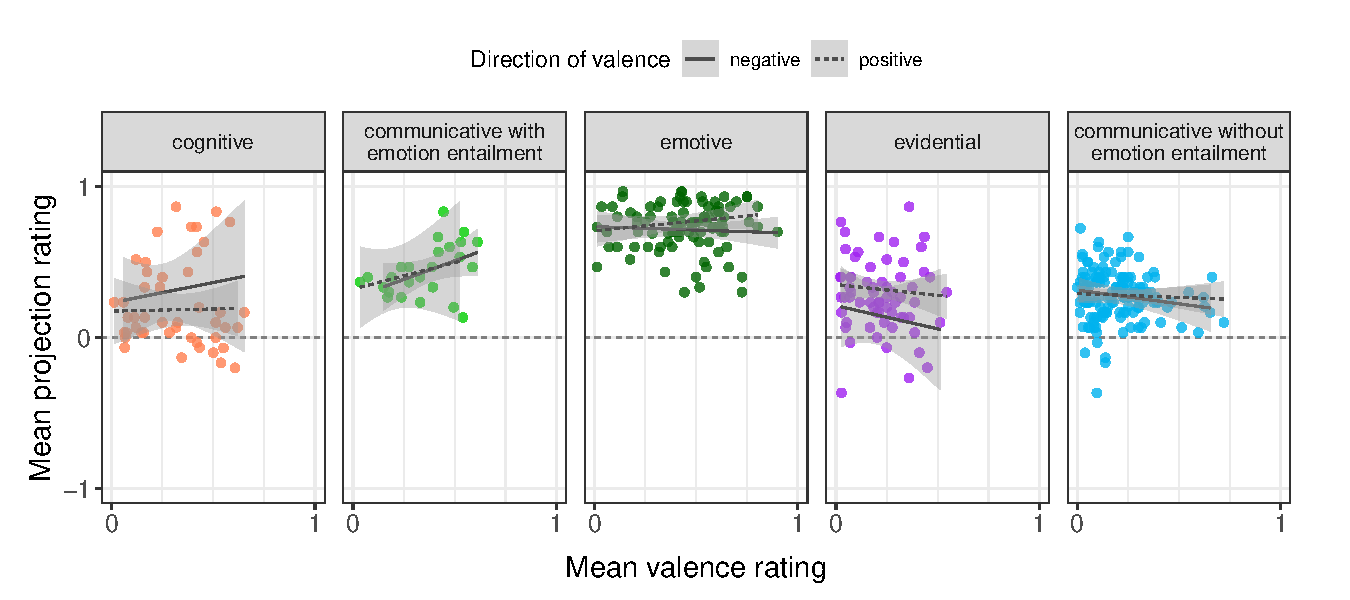
\includegraphics[width=1\textwidth]{projection-by-valence-faceted2}
	\caption{Mean projection rating by mean valence rating for each predicate type.}
	\label{projvalfac}
\end{figure}

Although higher dominance ratings are not generally associated with higher projection ratings, as shown in \figref{projVADdir} above, for the communicatives with an emotion entailment, dominance seems to be a highly significant predictor of projection ratings:
	
\begin{figure}[H]
	\centering
	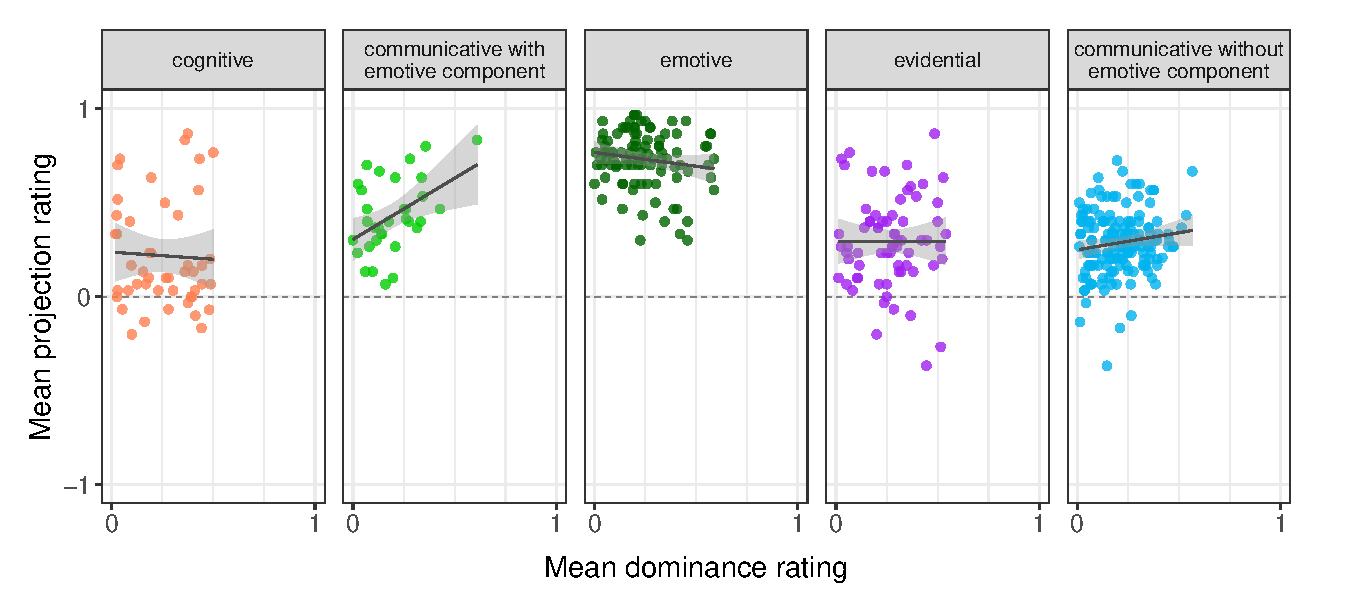
\includegraphics[width=1\textwidth]{projection-by-dominance-faceted2}
	\caption{Mean projection rating by mean dominance rating for each predicate type.}
	\label{projdomfac}
\end{figure}

Another correlation between projection and VAD ratings is the direction of valence: negative valence is associated with higher projection ratings compared to positive valence. A cumulative link mixed model fitted with the R package ``ordinal” predicting projection ratings from direction of valence with random intercepts for participant and entailment-cancelling environment identifies an effect of direction of valence on projection ratings at the 0.001 significance level.

\subsubsection{Sub-classification}

Although the presence of an emotion entailment in communicative predicates is positively correlated with higher projection ratings, the very wide range of projection ratings of the individual predicates shown in \figref{projemocomm} indicates that this entailment alone does not explain the high projection ratings of many members of this group of communicative predicates.

\begin{figure}[H]
	\centering
	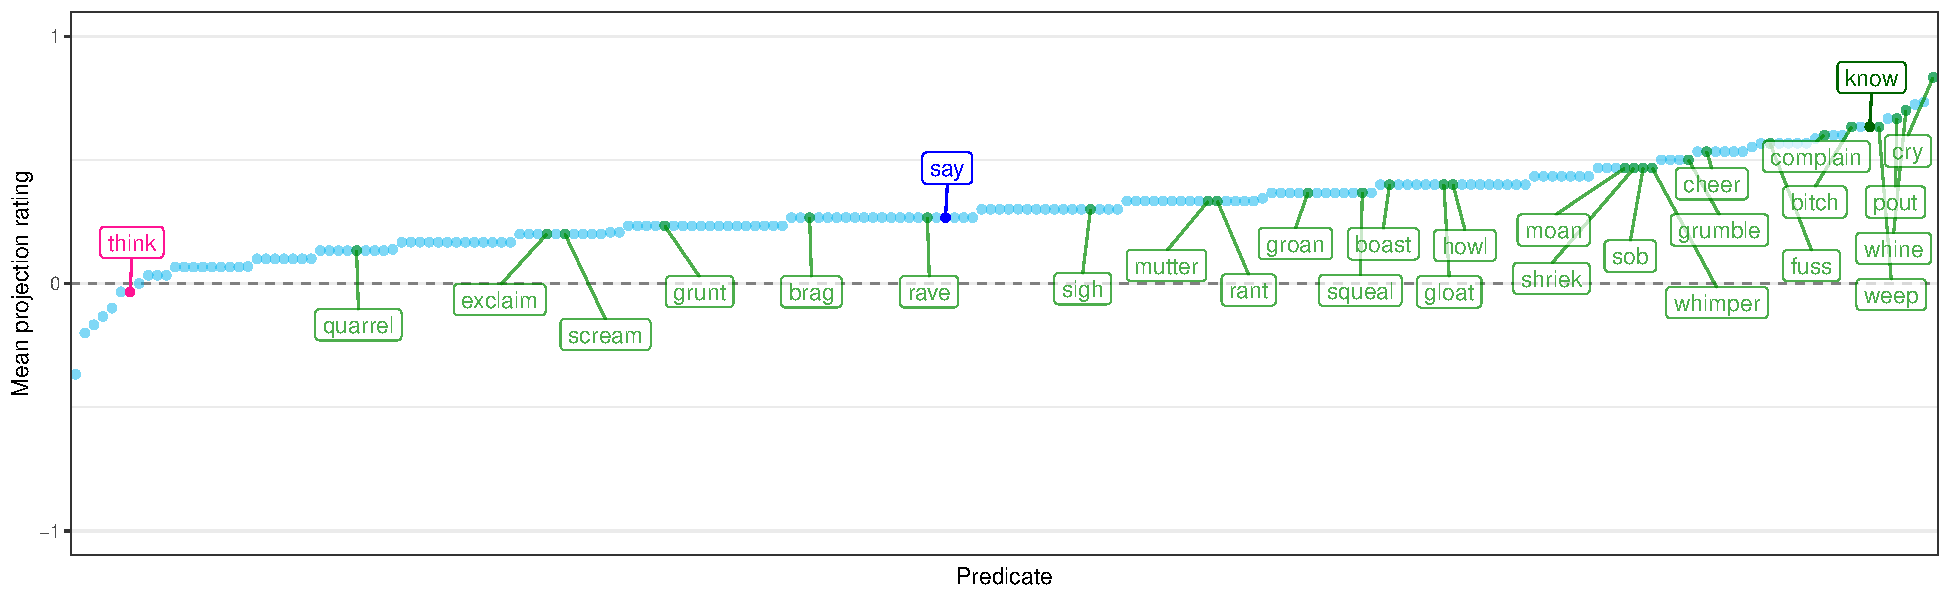
\includegraphics[width=1\textwidth]{projection-by-communicative-emoComms}
	\caption{Mean projection rating by communicative predicate with communicatives with an emotion entailment labelled in green. The cognitives \emph{think} and \emph{know} are included for reference.}
	\label{projemocomm}
\end{figure}

\noindent Further important entailments of communicative predicates are
\begin{itemize}
	\item The communication entailment:
	\begin{itemize}
		\item Part of all communicatives.
		\item The CC is communicated in some way.
		\item For many communicatives with an emotive component, this entailment seems to project when the predicate is stressed.
	\end{itemize}
	\item -	The belief entailment:
	\begin{itemize}
		\item Part only of some communicatives, including those with an emotion entailment.
		\item If the subject truly has an emotion about the CC, then they must also believe it. 
	\end{itemize}
	\item The manner entailment:
	\begin{itemize}
		\item Part of some of the communicatives with an emotion entailment, roughly \citepos{levin1993} ``verbs of manner of speaking”, such as \emph{groan}, \emph{moan} and \emph{squeal}.
		\item ``... distinguished from each other by the manner in which the sound is expressed.” (\citealt{levin1993}: 206)
	\end{itemize}
	\item The speaker attitude / evaluation (???) entailment:
	\begin{itemize}
		\item Part of some of the communicatives with an emotion entailment, roughly \citepos{levin1993} ``complain verbs”, like \emph{boast}, \emph{brag} and \emph{complain}.
		\item ``... specify the speaker’s attitude or feelings towards what is said.” (\citealt{levin1993}: 211)
	\end{itemize}
\end{itemize}

There are of course many more subtypes of communicative predicates to be identified. \figref{projcommextr} shows that on both ends of the projection rating range some subtypes of communicatives can be identified: 

\begin{figure}[H]
	\centering
	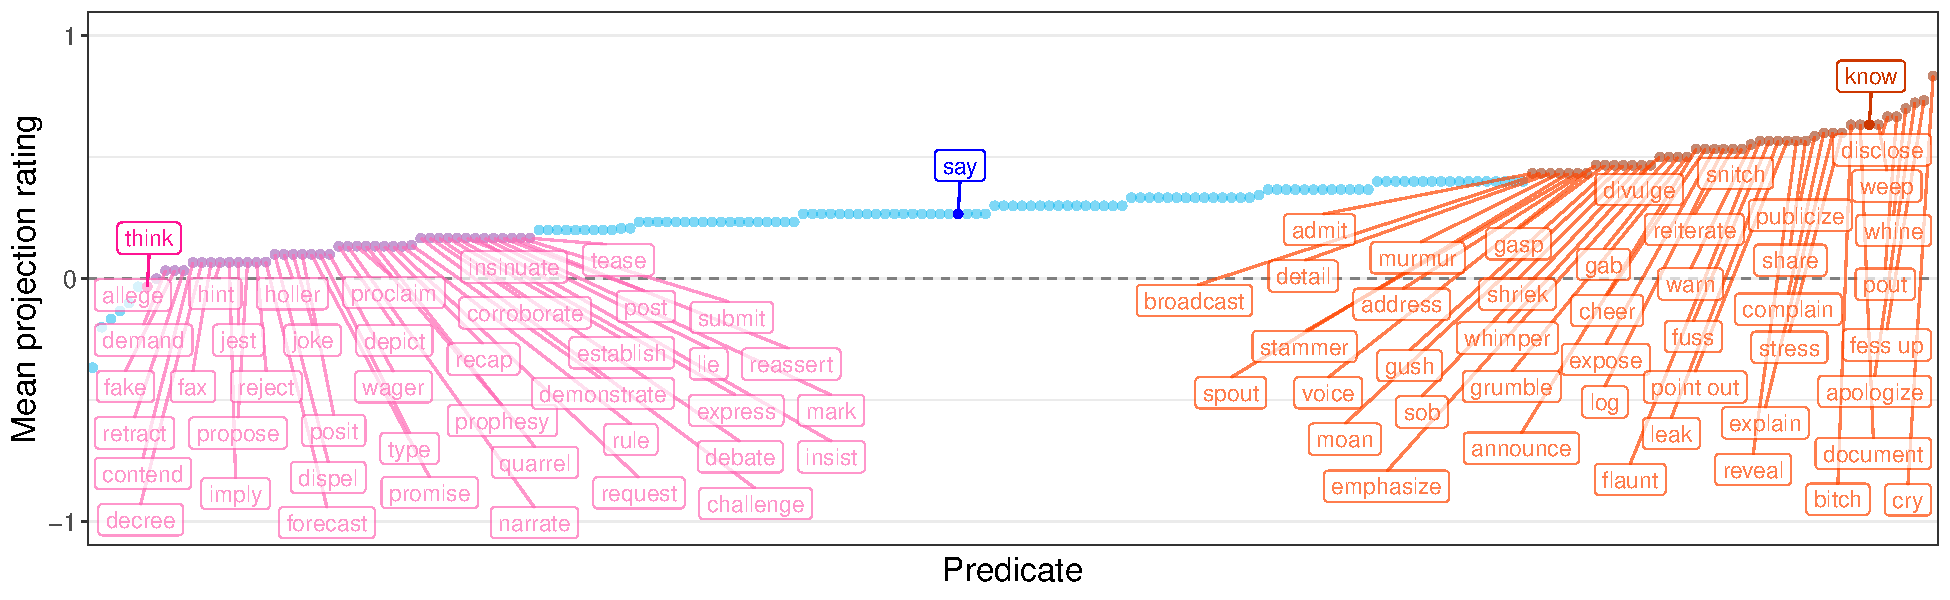
\includegraphics[width=1\textwidth]{projection-by-communicative-extremes-41-44}
	\caption{Mean projection rating by communicative predicate with labels for predicates with lowest and highest projection ratings. The cognitives \emph{think} and \emph{know} are included for reference.}
	\label{projcommextr}
\end{figure}

\noindent For this investigation, the next steps are the following:
\begin{itemize}
	\item Identify all members of these subtype-groups, including those that might not be on the end of the projection rating range where the group was identified.
	\item Define the set of the most important entailments for each group.
	\item Select a few interesting groups.
	\item Collect projection, acceptability and entailment ratings for some or all members of these groups.
\end{itemize}


\section{Experiments}
\subsection{Experiment 1}
\subsubsection{Projection ratings}
A closer inspection of participants’ acceptability ratings in the MV dataset reveals that these seem highly subjective, which calls into question the reliability of their projection ratings:
\begin{itemize}
	\item Only four of the 544 predicates in the MV dataset have mean acceptability ratings of less than 3. 
	\item Even for the least acceptable predicates, most individual ratings are somewhere in the middle and some even on the high end of the scale. This indicates that many participants considered a stimulus acceptable if it was interpretable (e.g. \emph{John was overheard that a particular thing happened.} $\approx$ \emph{John was overheard saying that a particular thing happened.}) 
	\item It therefore seems plausible that some veridicality and projection ratings might be based on utterances that differ from the original stimulus in unpredictable ways. 
	\item As a result, I have to collect my own projection ratings for the 201 communicatives investigated here.
\end{itemize}

The purpose of this experiment is to find possible additional evidence for the patterns in the MV dataset described above. Therefore, the stimuli used here are designed to be comparable to the MV stimuli, just with ‘a little bit more content’, i.e., the utterances are something that people would actually say or hear, unlike \citepos{white-rawlins-nels2018} rather artificial ``low context items”. The stimuli are like those in \cite{white-rawlins-nels2018} in that 
\begin{itemize}
	\item The past tense is used both for the matrix clause and the complement.
	\item The complement describes an event, not a state.
	\item The complement consists of a ``particular thing”, which here is realised as a definite DP, and an unaccusative verb.
	\item The complement does not contain aspect or mood marking.
\end{itemize}

However, for some of the communicatives in the MV dataset considered here, applying these rules would result in ungrammatical utterances. The following 10 predicates are therefore not included in this experiment:
\begin{itemize}
	\item \emph{decree}, \emph{demand}, \emph{dictate}, \emph{ordain}, \emph{request} and \emph{rule} require a subjunctive mood complement.
	\item \emph{forecast}, \emph{foretell}, \emph{predict} and \emph{prophesy} do not combine with a past tense complement.
\end{itemize}

For most of the remaining communicatives, it seems that they combine reasonably well with complements based on the rules above. Therefore, the following 11 complement clauses are used for the collection of projection ratings for these communicative predicates:
\begin{exe}
	\ex
	\begin{xlist}
		\ex The balloon popped.
		\ex The airbag deployed.
		\ex The bolt loosened.
		\ex The room darkened.
		\ex The computer restarted.
		\ex The sauce thickened.
		\ex The gate opened.
		\ex The factory closed.
		\ex The paper burnt.
		\ex The egg cracked.
		\ex The knot tightened.
	\end{xlist}
\end{exe}

These complement clauses are relatively neutral, i.e., not clearly positive or negative, to avoid mismatches with communicatives with an emotion entailment, as such unexpected combinations could affect whether the CC is perceived as projecting. At the same time, an emotional reaction to these CCs is still plausible. As the complement clause in \cite{white-rawlins-nels2018} describes an event, only complement clauses that cannot be interpreted as describing a state were used for this experiment. Sentences like, e.g., \emph{the fabric stretched}, which could also be interpreted as describing a property, in this case as \emph{the fabric was stretchable}, were therefore not used as complement clauses in this experiment. Since the predicate \emph{feign}, which refers to the subject's pretending to have a feeling or condition, is not compatible with the complement clauses above, this predicate is not included in the experiment, leaving 190 predicates to be investigated here. The cognitive predicates \emph{think} and \emph{know} are included in the experiment for reference. The total number of predicates is therefore 192.

The stimuli are created by randomly combining each of these complement clauses with a gender-neutral name and one of the predicates and then negating the resulting statement. For each of these utterances, participants are asked to judge whether the CC is true, as shown in (5a). 

\begin{exe}
	\ex
	\begin{xlist}
		\ex \emph{Reese didn't reply that the sauce thickened.} \\
		According to this statement, did the sauce thicken?
		\ex \emph{Alex didn't fall when the cane broke.} \\
		According to this statement, did the cane break?
		\ex \emph{Taylor smiled when the vase didn't shatter.} \\
		According to this statement, did the vase shatter?
	\end{xlist}
\end{exe}

In addition to the 11 trial items, each participant sees two control items, designed to elicit either a clear `yes' (5b) or a clear `no' (5c) response. For their responses participants use a slider marked 'no' at one end and 'yes' at the other, as shown in \figref{exquest} below.

\begin{figure}[H]
	\centering
	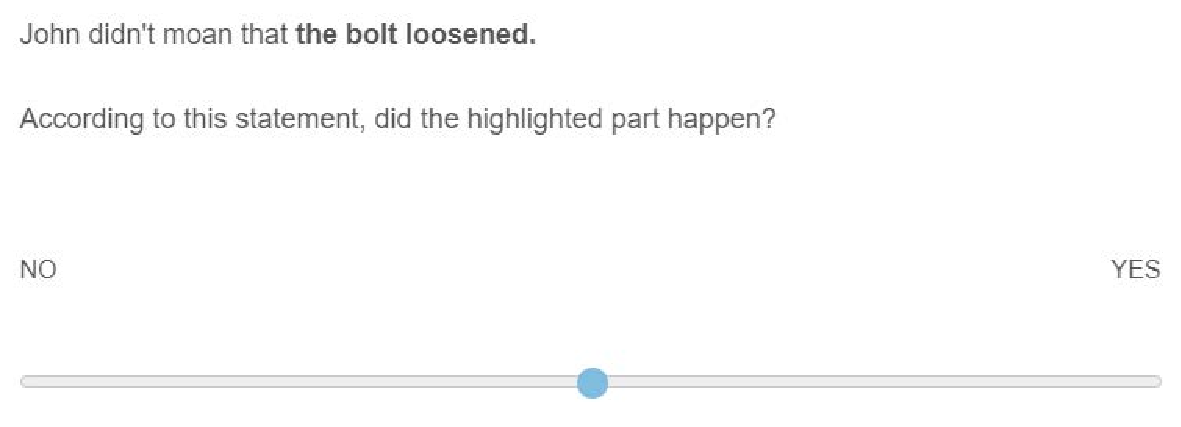
\includegraphics[width=0.4\textwidth]{example-question}
	\caption{Example stimulus for the collection of projection ratings.}
	\label{exquest}
\end{figure}

American spelling conventions were used for the stimuli, as the participants are native speakers of American English. To ensure that at least ten ratings per predicate are obtained, 350 participants are recruited via Prolific (192 predicates \(\times\) 20 ratings (10 \(\times\) 2, to be on the safe side) \(\div\) 11 ratings per participant \(\approx\) 349 participants). Each participant is paid £0.39 for taking part in the experiment, which takes approximately 2.5 minutes to complete.

...

\subsection{Experiment 2}
\subsubsection{Entailment ratings}

...

\subsubsection{Projection ratings}

Because the interpretation of some of these predicates is affected by focus, getting entailment and projection ratings for the same predicates from the same participants is desirable in these cases. If the communication entailment projects, the predicate was most likely read in a stressed manner.

...


\pagebreak

\bibliographystyle{../cslipubs-natbib}
\bibliography{../bibliography}


\end{document}
